\pdfminorversion=4
\documentclass[aspectratio=169]{beamer}
\usepackage{animate} % for animation
\usepackage{array,multirow,graphicx}
\usepackage{multicol}
\usepackage{etoolbox}
\graphicspath{{gambar/}}
\setbeamertemplate{caption}[numbered]
\setbeamertemplate{section in toc}[sections numbered]

% Hide subsubsections from TOC, but keep PDF bookmarks with beamer
\hypersetup{bookmarksopen=true,bookmarksopenlevel=4}
\setcounter{tocdepth}{4}

\renewcommand{\figurename}{Gambar.}
\renewcommand{\tablename}{Tabel.}

\usetheme[pageofpages=of,	% String used between the current page and the
							% total page count.
			alternativetitlepage=true,% Use the fancy title page.
			titleline=true,
			titlepagelogo=OK-LOGO-ITK.jpg
%          	 titlepagelogo=fig/jaist_logo.png
			]{Torino}
			% change /beamerinnerthemefancy.sty to resize the logo
\usecolortheme{freewilly}

\makeatletter
\patchcmd{\beamer@sectionintoc}{\vskip1.5em}{\vskip0em}{}{}
\makeatother

\author{Mifta Nur Farid, S.T., M.T. \\
	miftanurfarid@lecturer.itk.ac.id}
\title{RANGKAIAN ELEKTRONIKA II}
\subtitle{Penguat Diferensial}
\institute{Teknik Elektro \\ Institut Teknologi Kalimantan \\ Balikpapan, Indonesia}
\date{\tiny Februari 22, 2021}

% The log drawn in the upper right corner.
\logo{
\includegraphics[height=0.13\paperheight]{OK-LOGO-ITK.jpg}}

\begin{document}

\begin{frame}[t,plain]
\titlepage
\end{frame}

%\begin{frame}{Bahan Kajian}
%	\begin{multicols}{2} % Two columns for outline
%    \tableofcontents[subsectionstyle=hide]
%	\end{multicols}
%\end{frame}

\section{Pengantar}
\begin{frame}{Pengantar}
	\begin{itemize}
		\item Istilah Operational amplifier (op-amp) merujuk kepada sebuah amplifier/penguat yang menjalankan suatu operasi matematika.
		\item Dalam sejarahnya, op-amp pertama digunakan di dalam komputer analog untuk melakukan operasi penjumlahan, perkalian dan lainnya.
		\item Op-amp dibuat sebagai sirkuit diskrit $ \rightarrow $ sekarang kebanyakan op-amp adalah sirkuit terintegrasi/ integrated circuits (IC). 
	\end{itemize}
\end{frame}

\begin{frame}{Pengantar}
	\begin{figure}
		\centering
		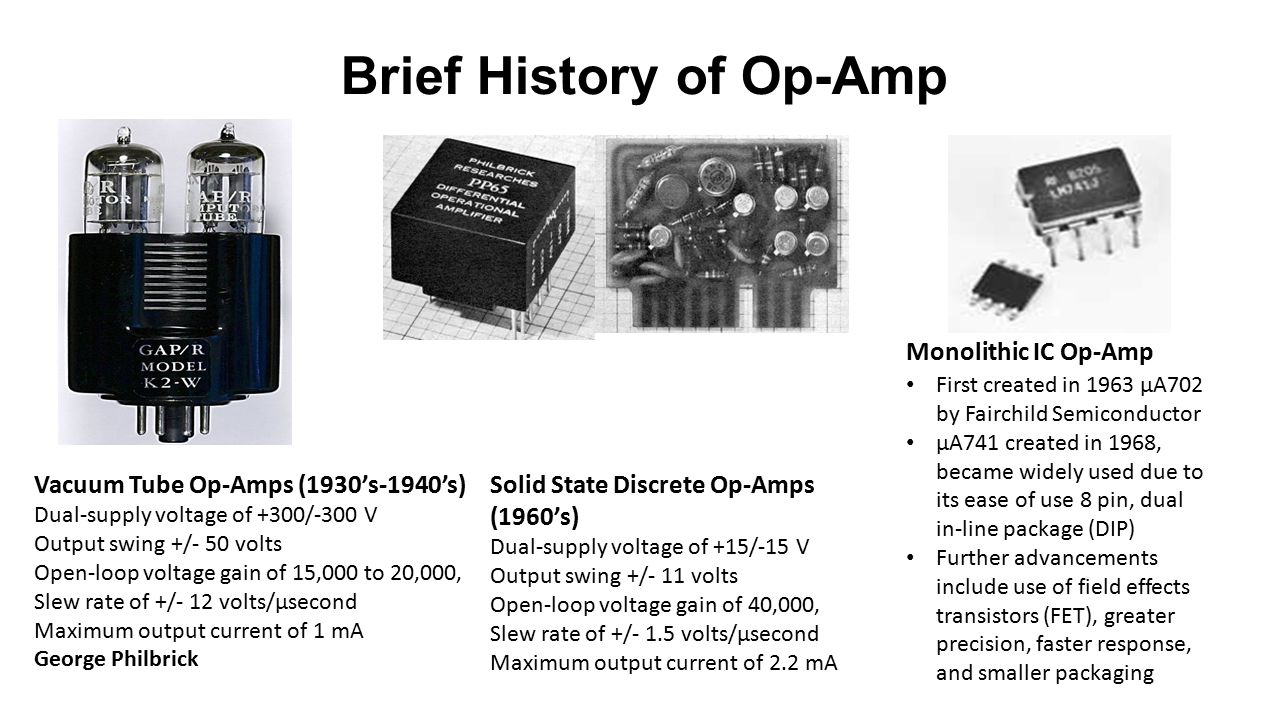
\includegraphics[height=0.75\textheight]{gambar/01.history-op-amp}
		\caption{Perkembangan op-amp}
		\label{fig:history-op-amp}
	\end{figure}
\end{frame}

\begin{frame}{Pengantar}
	\begin{itemize}
		\item Op-amp $ \rightarrow $ penguat DC/DC amplifier dengan voltage gain/penguatan tegangan yang sangat besar, impendansi input yang sangat besar, dan impedansi output yang sangat kecil.
		\item Frekuensi unity gain dari 1 hingga lebih dari 20 Mhz.
		\item IC op-amp adalah sebuah blok fungsional yang lengkap dengan pin eksternal.
		\item Hanya dengan menghubungkan pin tersebut ke suplai tegangan dan beberapa komponen, kita dapat dengan cepat membuat segala jenis rangkaian yang berguna.
	\end{itemize}
\end{frame}

\begin{frame}{Pengantar}
	\begin{itemize}
		\item Rangkaian input yang paling banyak digunakan di op-amp adalah sebuah penguat diferensial/ differential amplifier.
		\item Konfigurasi dari penguat ini memberikan banyak karakteristik input di IC.
		\item Penguat diferensial juga dapat dikonfigurasi dalam bentuk diskrit untuk digunakan dalam komunikasi, instrumentasi, dan rangkaian kontrol industri.
		\item \textbf{Kita akan fokus pada penguat diferensial yang digunakan dalam IC.}
	\end{itemize}
\end{frame}

\begin{frame}{Pengantar}
	\begin{itemize}
		\item Sub-CPMK:
		\begin{itemize}
			\item Mahasiswa mampu menganalisis rangkaian penguat diferensial (C4, P3, A3)
		\end{itemize}
		\item Bahan Kajian
		\begin{enumerate}
			\item Konsep dasar penguat diferensial;
			\item Analisis DC dari penguat diferensial;
			\item Analisis AC dari penguat diferensial;
			\item Common‐mode gain;
		\end{enumerate}
	\end{itemize}
\end{frame}

\section{Penguat Diferensial}
\begin{frame}{Penguat Diferensial}
	\begin{enumerate}
		\item Transistor, dioda, dan resistor adalah komponen-komponen praktis yang ada di dalam IC.
		\item Kapasitor mungkin dapat digunakan, tapi ukurannya sangat kecil, $ < $ 50 pF.
		\item Sehingga tidak bisa menggunakan kapasitor kopling dan  kapasistor bypass seperti pada rangkaian diskret.
		\item Harus menggunakan kopling langsung antara stage-nya + menghilangkan kapasitor bypass emitter.
		\item Solusinya? $ \rightarrow $ penguat diferensial
		\item Penguat diferensial $ \rightarrow $ menghilangkan kebutuhan terhadap kapasitor bypass emitter
		\item Penguat diferensial $ \leftarrow $ banyak digunakan sebagai input stage hampir di setiap IC op-amp
	\end{enumerate}
\end{frame}

\subsection{Differential Input dan Output}
\begin{frame}{Difderential Input dan Output}
	\begin{multicols}{2}
		\begin{figure}
			\centering
			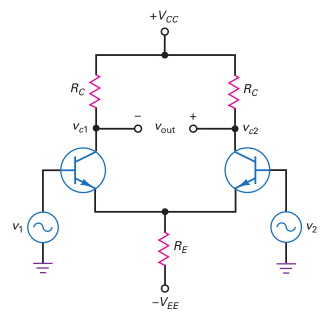
\includegraphics[height=0.7\textheight]{gambar/01.differential_input_output}
		\end{figure}
		\columnbreak
		\begin{itemize}
			\item Ada 2 CE stage yang paralel terhadap resistor \textit{common emitter} $ R_E $
			\item Meskipun ada 2 tegangan \textit{input} ($ v_1 \text{, } v_2$) dan 2 tegangan \textit{collector} ($ v_{c1} \text{, } v_{c2}$), keseluruhan rangkaian dianggap 1 stage.
			\item Tidak ada kapasitor kopling dan bypass $ \rightarrow $ tidak ada lower cutoff frequency
		\end{itemize}
	\end{multicols}
\end{frame}

\begin{frame}{Diferential Input dan Output}
	\begin{multicols}{2}
		\begin{figure}
			\centering
			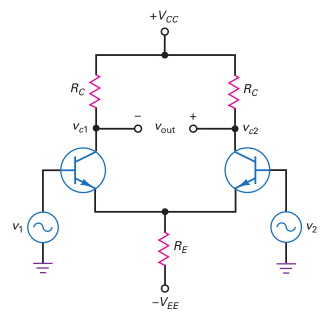
\includegraphics[height=0.7\textheight]{gambar/01.differential_input_output}
		\end{figure}
		\columnbreak
		\begin{itemize}
			\item Tegangan output AC :\\
			
			\begin{equation} \label{pers.1}
				v_{out} =  v_{c2} - v_{c1}
			\end{equation}
		
			\item $ v_{out} $ = differential output, karena menggabungkan 2 tegangan collector.
			\item Transistor yang identik + resistor collector yang sama $ \rightarrow $ ideal
			\item $ v_1 = v_2 \rightarrow v_{out} = 0 $
			\item $ v_1 > v_2 \rightarrow v_{out} $ memiliki polaritas seperti gambar di samping.
			\item $ v_1 < v_2 \rightarrow v_{out} $ inverted + polaritas yang berkebalikan
		\end{itemize}
	\end{multicols}
\end{frame}

\begin{frame}{Diferential Input dan Output}
	\begin{multicols}{2}
		\begin{figure}
			\centering
			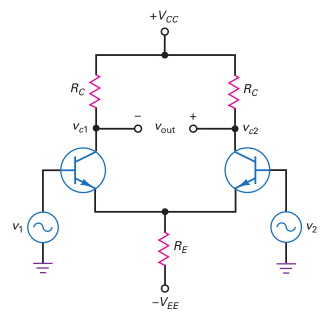
\includegraphics[height=0.7\textheight]{gambar/01.differential_input_output}
		\end{figure}
		\columnbreak
		\begin{itemize}
			\item $ v_1 $ = \textbf{noninverting input} karena $ v_{out} $ memiliki fasa yang sama dengan $ v_1 $
			\item $ v_2 $ = \textbf{inverting input} karena $ v_{out} $ memiliki fasa yang berbeda 180 $ ^{\circ} $ dengan $ v_2 $
			\item Terkadang, noninverting input yang digunakan dan  inverting input di-grounding, terkadang juga sebaliknya.
		\end{itemize}
	\end{multicols}
\end{frame}

\begin{frame}{Diferential Input dan Output}
	\begin{multicols}{2}
		\begin{figure}
			\centering
			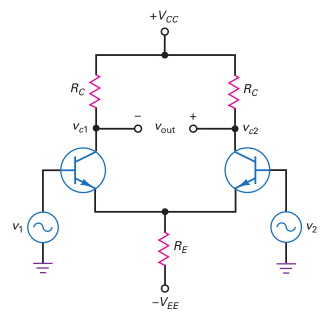
\includegraphics[height=0.7\textheight]{gambar/01.differential_input_output}
		\end{figure}
		\columnbreak
		\begin{itemize}
			\item Jika kedua input-nya ada, input totalnya disebut differential input karena tegangan output sama dengan penguatan tegangan (voltage gain) $ \times $ selisih dari kedua tegangan input.
			\begin{equation} \label{pers.2}
				v_{out} = A_v (v_1 - v_2)
			\end{equation}
			\item $ A_v $ = penguatan tegangan/ voltage gain
		\end{itemize}
	\end{multicols}
\end{frame}

\subsection{Single-Ended Output}
\begin{frame}{Single-Ended Output}
	\begin{multicols}{2}
		\begin{figure}
			\centering
			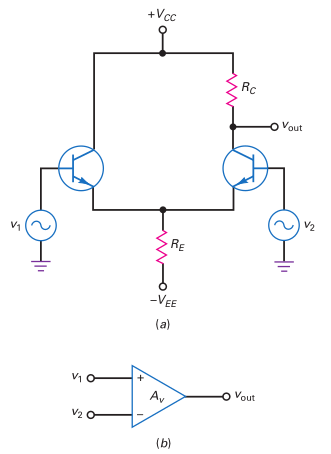
\includegraphics[height=0.8\textheight]{gambar/01.diferential_input_single_ended}
		\end{figure}
		\columnbreak
		\begin{itemize}
			\item Differential output (gambar sebelumnya) membutuhkan floating load, karena kedua ujung dari load tidak ke ground.
			\item Umumnya, load/ beban adalah single-ended, salah satu ujungnya ke ground. Seperti pada gambar (a).
			\item $ v_{out} = A_v (v_1 - v_2) $, tapi voltage gain ($ A_v $) hanya setengah
			\item Blok-diagram, gambar (b), sama dengan op-amp
		\end{itemize}
	\end{multicols}
\end{frame}

\begin{frame}{Konfigurasi Noninverting-Input}
	\begin{multicols}{2}
		\begin{center}
			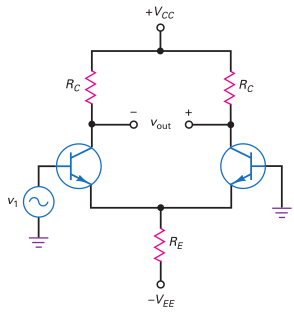
\includegraphics[height=0.7\textheight]{gambar/01.noninverting_input+differential_output}
		\end{center}
		\columnbreak
		\begin{itemize}
			\item Konfigurasi ini memiliki
			\begin{itemize}
				\item Noninverting input
				\item Differential output
			\end{itemize}
			\item Karena $ v_2 = 0 $, maka
		\end{itemize}
		\begin{equation} \label{pers.3}
			v_{out} = A_v (v_1)
		\end{equation}
	\end{multicols}
\end{frame}

\begin{frame}{Konfigurasi Noninverting-Input}
	\begin{multicols}{2}
		\begin{center}
			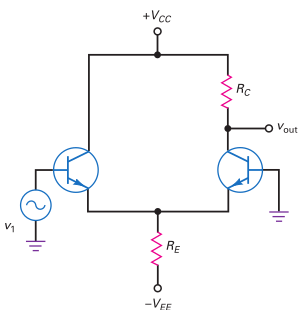
\includegraphics[height=0.7\textheight]{gambar/01.noninverting_input+single-ended_output}
		\end{center}
		\columnbreak
		\begin{itemize}
			\item Konfigurasi ini memiliki
			\begin{itemize}
				\item Noninverting input
				\item Single-ended output
			\end{itemize}
			\item Karena $ v_{out} $ adalah tegangan output AC, maka $ v_{out} $ tetap sama seperti sebelumnya yaitu $ v_{out} = A_v (v_1) $
		\end{itemize}
		\begin{itemize}
			\item Tapi $ A_v $ akan bernilai setengahnya karena output hanya diambil dari satu sisi dari diff-amp
		\end{itemize}
	\end{multicols}
\end{frame}

\subsection{Konfigurasi Inverting-input}
\begin{frame}{Konfigurasi Inverting-input}
	\begin{multicols}{2}
		\begin{center}
			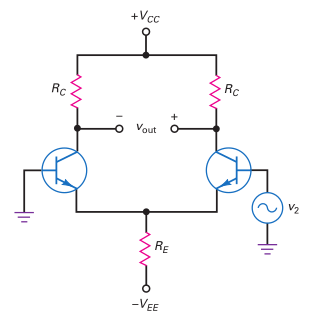
\includegraphics[height=0.7\textheight]{gambar/01.inverting_input+differential_output}
		\end{center}
		\columnbreak
		\begin{itemize}
			\item $ v_2 $ adalah active input dan $ v_1 $ adalah grounded input, maka
			\begin{equation} \label{pers.4}
				v_{out} = -A_v(v_2)
			\end{equation}
			\item Tanda minus (-) menunjukkan fasa yang berkebalikan
		\end{itemize}
	\end{multicols}
\end{frame}

\begin{frame}{Konfigurasi Inverting-input}
	\begin{multicols}{2}
		\begin{center}
			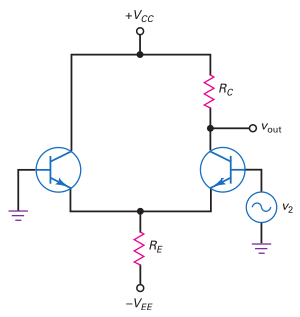
\includegraphics[height=0.7\textheight]{gambar/01.inverting_input+single-ended_output}
		\end{center}
		\columnbreak
		\begin{itemize}
			\item Tegangan output juga sama dengan sebelumnya, yaitu $ v_{out} = -A_v(v_2) $
		\end{itemize}
	\end{multicols}
\end{frame}

\subsection{Ringkasan}
\begin{frame}{Ringkasan}
	\begin{center}
		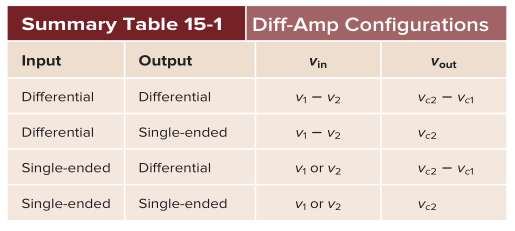
\includegraphics[height=0.6\textheight]{gambar/01.ringkasan_dif-amp-conf}
	\end{center}
\end{frame}

\section{Analisis DC dari Diff Amp}
\begin{frame}{Analisis DC dari Diff Amp}
	\begin{multicols}{2}
		\begin{center}
			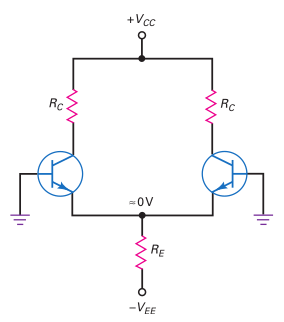
\includegraphics[width=0.7\textheight]{gambar/01.ideal_dc_analysis}
		\end{center}
		\columnbreak
		\begin{itemize}
			\item Rangkaian ekivalen DC dari diff amp.
			\item Pada pembahasan berikutnya, kita akan mengasumsikan transistornya identik dan resistor collectornya sama.
			\item Kita asumsikan juga kedua base di-grounded
		\end{itemize}
	\end{multicols}
\end{frame}

\subsection{Analisis Ideal}
\begin{frame}{Analisis Ideal}
	\begin{multicols}{2}
		\begin{center}
			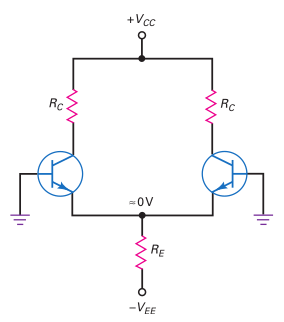
\includegraphics[width=0.7\textheight]{gambar/01.ideal_dc_analysis}
		\end{center}
		\columnbreak
		\begin{itemize}
			\item Diff amp disebut juga long-tail pair karena kedua transistor saling berbagi satu common resistor $ R_E $.
			\item Arus yang mengalir melalui common resistor ini disebut tail current.
			\item Jika kita mengabaikan $ V_{BE} $ drop sepanjang dioda emitter, maka di atas emitter resistor idealnya adalah sebuah titik ground DC.
		\end{itemize}
		\vfill\null
	\end{multicols}
\end{frame}

\begin{frame}{Analisis Ideal}
	\begin{multicols}{2}
		\begin{center}
			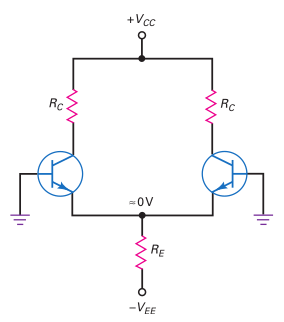
\includegraphics[width=0.7\textheight]{gambar/01.ideal_dc_analysis}
		\end{center}
		\columnbreak
		\begin{itemize}
			\item Sehingga semua $ V_{EE} $ ada di seberang $ R_E $ dan arus tail bernilai
			\begin{equation} \label{pers.5}
				I_T = \frac{V_{EE}}{R_E}
			\end{equation}
			\item Ketika keduanya benar-benar sama, maka arus tail akan terbagi sama, sehingga tiap transistor memiliki arus emitter sebesar \\
			\begin{equation} \label{pers.6}
				I_{EE} = \frac{I_T}{2}
			\end{equation}
		\end{itemize}
		\vfill\null
	\end{multicols}
\end{frame}

\begin{frame}{Analisis Ideal}
	\begin{multicols}{2}
		\begin{center}
			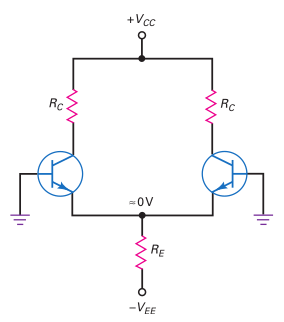
\includegraphics[width=0.7\textheight]{gambar/01.ideal_dc_analysis}
		\end{center}
		\columnbreak
		\begin{itemize}
			\item Tegangan DC pada kedua collector sebesar \\
			\begin{equation} \label{pers.7}
				V_C = V_{CC} - I_C R_C
			\end{equation}
		\end{itemize}
		\vfill\null
	\end{multicols}
\end{frame}

\subsection{Metode Perkiraan Kedua}
\begin{frame}{Metode perkiraan kedua}
	\begin{multicols}{2}
		\begin{center}
			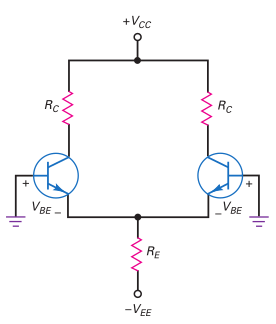
\includegraphics[width=0.7\textheight]{gambar/01.second_approximation}
		\end{center}
		\columnbreak
		\begin{itemize}
			\item Kita bisa meningkatkan analisis DC dengan cara menyertakan $ V_{BE} $ drop di setiap dioda emitter
			\begin{equation} \label{pers.8}
				I_T = \frac{V_{EE} - V_{BE}}{R_E}
			\end{equation}
			dimana $ V_{BE} = 0.7 $ V untuk transistor silikon.
		\end{itemize}
		\vfill\null
	\end{multicols}
\end{frame}

\subsection{Contoh Soal 1.1}
\begin{frame}{Contoh Soal 1.1}
	\begin{multicols}{2}
		\begin{center}
			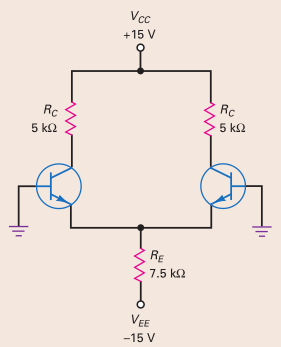
\includegraphics[width=0.6\textheight]{gambar/01.latihan_soal_1a}
		\end{center}
		\columnbreak
		\begin{itemize}
			\item Pertanyaan:
			\begin{itemize}
				\item Berapa arus dan tegangan ideal dari gambar di samping?
			\end{itemize}
			\item Jawaban:
			\begin{itemize}
				\item Berdasarkan persamaan \ref{pers.5}, arus tail adalah:
				\[I_T = \frac{V_{EE}}{R_E} = \frac{15 \text{ v }}{7.5 \text{ k}\Omega} = 2 \text{ mA} \]
				\item Tiap arus emitter adalah separuh dari arus tail:
				\[ I_E = \frac{I_T}{2} = \frac{2 \text{ mA}}{2} = 1 \text{ mA} \]
			\end{itemize}
		\end{itemize}
		\vfill\null
	\end{multicols}
\end{frame}

\begin{frame}{Contoh Soal 1.1}
	\begin{multicols}{2}
		\begin{center}
			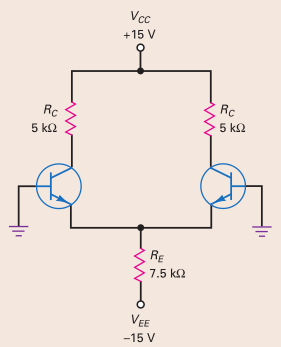
\includegraphics[width=0.6\textheight]{gambar/01.latihan_soal_1a}
		\end{center}
		\columnbreak
		\begin{itemize}
			\item Jawaban:
			\begin{itemize}
				\item Setiap tegangan collectornya adalah:
				\begin{align*}
					V_C &= V_{CC} - I_C R_C \\
					&= 15 \text{ V} - (1 \text{ mA})(5 \text{ k}\Omega) \\
					&= 10 \text{ V}
				\end{align*}
				\[  \]
			\end{itemize}
		\end{itemize}
		\vfill\null
	\end{multicols}
\end{frame}

\subsection{Latihan Soal 1.1}
\begin{frame}{Latihan Soal 1.1}
	\begin{multicols}{2}
		\begin{center}
			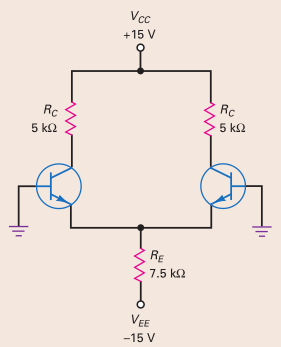
\includegraphics[width=0.6\textheight]{gambar/01.latihan_soal_1a}
		\end{center}
		\columnbreak
		\begin{itemize}
			\item Pertanyaan:
			\begin{itemize}
				\item Berapa arus dan tegangan ideal jika $ R_E = 5 \text{ k}\Omega $
			\end{itemize}
			\item Jawaban: ??
			\begin{itemize}
				\item \textit{Silakan dikerjakan}
			\end{itemize}
		\end{itemize}
		\vfill\null
	\end{multicols}
\end{frame}

\subsection{Contoh Soal 1.2}
\begin{frame}{Contoh Soal 1.2}
	\begin{multicols}{2}
		\begin{center}
			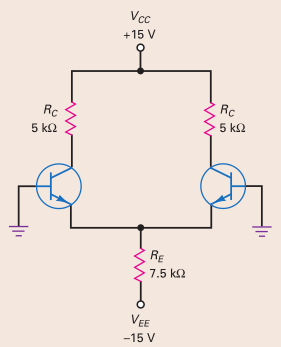
\includegraphics[width=0.6\textheight]{gambar/01.latihan_soal_1a}
		\end{center}
		\columnbreak
		\begin{itemize}
			\item Pertanyaan:
			\begin{itemize}
				\item Dengan menggunakan metode kedua, berapa arus dan tegangan ideal dari gambar di samping?
			\end{itemize}
			\item Jawaban:
			\begin{itemize}
				\item Arus tail-nya adalah:
				\begin{align*}
					I_T &= \frac{V_{EE}-V_{BE}}{R_E} = \frac{15 \text{ V} - 0.7 \text{ V}}{7.5 \text{ k}\Omega} \\
					&= 1.91 \text{ mA}
				\end{align*}
			\end{itemize}
		\end{itemize}
		\vfill\null
	\end{multicols}
\end{frame}

\begin{frame}{Contoh Soal 1.2}
	\begin{multicols}{2}
		\begin{center}
			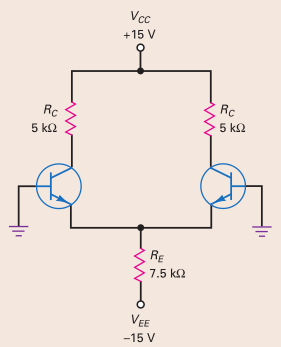
\includegraphics[width=0.6\textheight]{gambar/01.latihan_soal_1a}
		\end{center}
		\columnbreak
		\begin{itemize}
			\item Jawaban:
			\begin{itemize}
				\item Setiap arus emitternya adalah setengah dari arus tailnya:
				\[ I_E = \frac{I_T}{2} = \frac{1.91 \text{ mA}}{2} = 0.955 \text{ mA} \]
				\item Tegangan collectornya sebesar:
				\begin{align*}
					V_C &= V_{CC} - I_C R_C \\
					&= 15 \text{ V} - (0.955 \text{ mA})(5 \text{ k}\Omega) \\
					&= 10.2 \text{ V}
				\end{align*}
			\end{itemize}
		\end{itemize}
		\vfill\null
	\end{multicols}
\end{frame}

\subsection{Latihan Soal 1.2}
\begin{frame}{Latihan Soal 1.2}
	\begin{multicols}{2}
		\begin{center}
			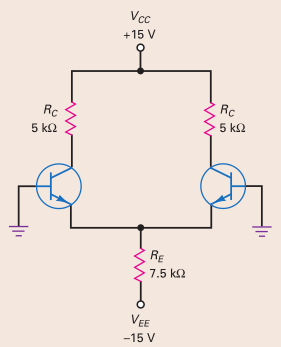
\includegraphics[width=0.6\textheight]{gambar/01.latihan_soal_1a}
		\end{center}
		\columnbreak
		\begin{itemize}
			\item Pertanyaan:
			\begin{itemize}
				\item Dengan menggunakan metode kedua, berapa arus dan teganan ideal jika $ R_E = 5 \text{ k}\Omega $
			\end{itemize}
			\item Jawaban:
			\begin{itemize}
				\item \textit{Silakan dikerjakan}
			\end{itemize}
		\end{itemize}
		\vfill\null
	\end{multicols}
\end{frame}

\subsection{Contoh Soal 1.3}
\begin{frame}{Contoh Soal 1.3}
	\begin{multicols}{2}
		\begin{center}
			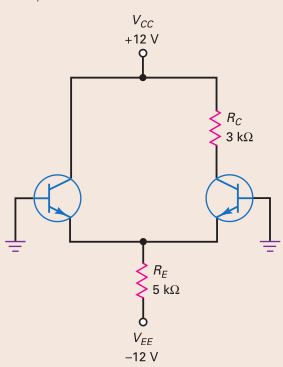
\includegraphics[width=0.6\textheight]{gambar/01.latihan_soal_3}
		\end{center}
		\columnbreak
		\begin{itemize}
			\item Pertanyaan:
			\begin{itemize}
				\item Berapa arus dan tegangan di dalam rangkaian single-ended output di samping
			\end{itemize}
			\item Jawaban:
			\begin{itemize}
				\item Idealnya, arus tail:
				\[ I_T = \frac{V_{EE}}{R_E} = \frac{12 \text{ V}}{5 \text{ kV}} = 2.4 \text{ mA} \]
				\item Setiap arus emitter adalah setengah dari arus tailnya:
				\[ I_E = \frac{I_T}{2} = \frac{2.4 \text{ mA}}{2} =1.2 \text{ mA} \]
			\end{itemize}
		\end{itemize}
		\vfill\null
	\end{multicols}
\end{frame}

\begin{frame}{Contoh Soal 1.3}
	\begin{multicols}{2}
		\begin{center}
			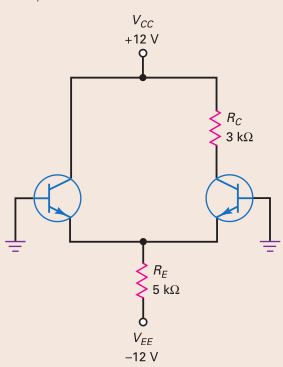
\includegraphics[width=0.6\textheight]{gambar/01.latihan_soal_3}
		\end{center}
		\columnbreak
		\begin{itemize}
			\item Jawaban:
			\begin{itemize}
				\item Tegangan collector yang sebelah kanan adalah:
				\begin{align*}
					V_C &= V_{CC} - I_C R_C \\
					&= 12 \text{ V} - (1.2 \text{ mA})(3 \text{ k}\Omega) \\
					&= 8.4 \text{ V}
				\end{align*}
				\item Sedangkan tegangan collector sebelah kiri adalah 12 V.
			\end{itemize}
		\end{itemize}
		\vfill\null
	\end{multicols}
\end{frame}

\begin{frame}{Contoh Soal 1.3}
	\begin{multicols}{2}
		\begin{center}
			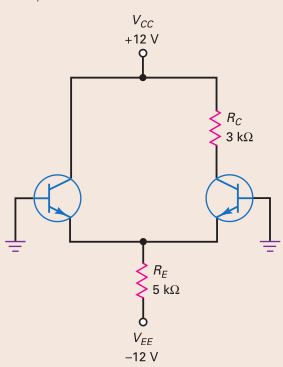
\includegraphics[width=0.6\textheight]{gambar/01.latihan_soal_3}
		\end{center}
		\columnbreak
		\begin{itemize}
			\item Jawaban:
			\begin{itemize}
				\item Jika kita gunakan metode yang kedua, kita dapatkan:
				\begin{align*}
					I_T &= \frac{V_{EE} - V_{BE}}{R_E} \\
					&= \frac{12 \text{ V} - 0.7 \text{ V}}{5 \text{ k}\Omega} \\
					&= 2.26 \text{ mA} \\
					\\
					I_E &= \frac{I_T}{2} = \frac{2.26 \text{ mA}}{2} = 1.13 \text{ mA}
				\end{align*}
			\end{itemize}
		\end{itemize}
		\vfill\null
	\end{multicols}
\end{frame}

\begin{frame}{Contoh Soal 1.3}
	\begin{multicols}{2}
		\begin{center}
			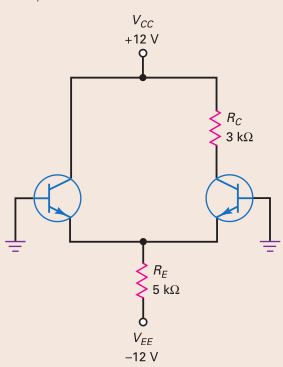
\includegraphics[width=0.6\textheight]{gambar/01.latihan_soal_3}
		\end{center}
		\columnbreak
		\begin{itemize}
			\item Jawaban:
			\begin{itemize}
				\item[]
				\begin{align*}
					V_C &= V_{CC} - I_C R_C \\
					&= 12 \text{ V} - (1.13 \text{ mA})(3 \text{ k}\Omega) \\
					&= 8.61 \text{ V}
				\end{align*}
			\end{itemize}
		\end{itemize}
		\vfill\null
	\end{multicols}
\end{frame}

\subsection{Latihan Soal 1.3}
\begin{frame}{Latihan Soal 1.3}
	\begin{multicols}{2}
		\begin{center}
			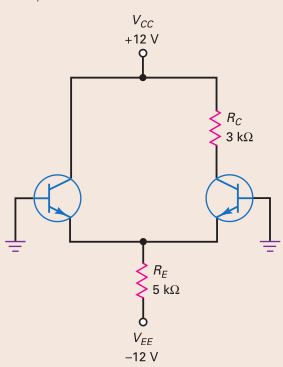
\includegraphics[width=0.6\textheight]{gambar/01.latihan_soal_3}
		\end{center}
		\columnbreak
		\begin{itemize}
			\item Pertanyaan:
			\begin{itemize}
				\item Jika $ R_E = 3 \text{ k}\Omega $, tentukan arus dan tegangan dengan menggunakan metode kedua.
			\end{itemize}
		\end{itemize}
		\vfill\null
	\end{multicols}
\end{frame}

\section{Analisis AC dari Diff Amp}
\begin{frame}{Analisis AC dari Diff Amp}
	\begin{itemize}
		\item Pada bagian ini, kita akan menurunkan persamaan untuk penguatan tegangan (voltage gain) dari diff amp.
		\item Kita mulai dengan konfigurasi yang paling sederhana, noninverting input dan single-ended output.
		\item Setelah menurunkan penguatan tegangan, kita akan kembangkan hasilnya ke konfigurasi yang lain.
	\end{itemize}
\end{frame}

\subsection{Teori Operasi}
\begin{frame}{Teori Operasi}
	\begin{multicols}{2}
		\begin{center}
			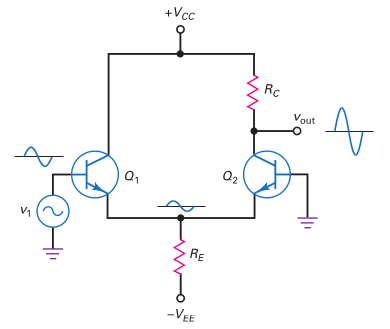
\includegraphics[height=0.7\textheight]{gambar/01.noninverting-input+single-ended-output_AC}
		\end{center}
		\columnbreak
		\begin{itemize}
			\item Gambar di samping adalah noninverting input dan single-ended output.
			\item Dengan $ R_E $ yang besar, arus tail hampir konstan saat ada sinyal AC yang kecil.
			\item Jika arus emitter di $ Q_1 $ meningkat maka arus emitter di  $ Q_2 $ menurun, dan sebaliknya.
		\end{itemize}
	\end{multicols}
\end{frame}

\begin{frame}{Teori Operasi}
	\begin{multicols}{2}
		\begin{center}
			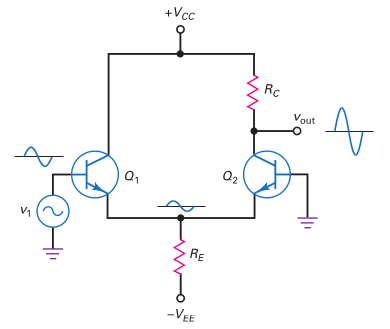
\includegraphics[height=0.7\textheight]{gambar/01.noninverting-input+single-ended-output_AC}
		\end{center}
		\columnbreak
		\begin{itemize}
			\item Transistor $ Q_1 $ bertindak seperti emitter follower yang menghasilkan tegangan AC di seberang resistor emitter.
			\item Tegangan AC ini bernilai setengah dari tegangan input $ v_1 $
			\item Pada setengah siklus positif dari tegangan input, arus emitter $ Q_1 $ meningkat, arus emitter $ Q_2 $ menurun, dan tegangan collector $ Q_2 $ meningkat.
		\end{itemize}
	\end{multicols}
\end{frame}

\begin{frame}{Teori Operasi}
	\begin{multicols}{2}
		\begin{center}
			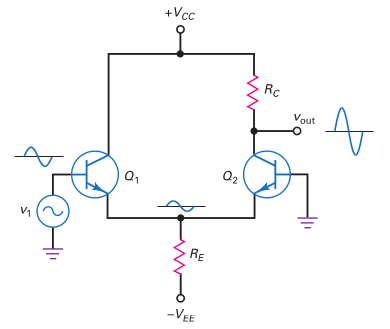
\includegraphics[height=0.7\textheight]{gambar/01.noninverting-input+single-ended-output_AC}
		\end{center}
		\columnbreak
		\begin{itemize}
			\item Sama halnya pada setengah siklus negatif dari tegangan input, arus emitter $ Q_1 $ menurun, arus emitter $ Q_2 $ meningkat, dan tegangan collector $ Q_2 $ menurun.
			\item Hal ini yang menyebabkan gelombang sinus yang dikuatkan memiliki fasa yang sama dengan noninverting input.
		\end{itemize}
	\end{multicols}
\end{frame}

\subsection{Single-Ended Output Gain}
\begin{frame}{Single-ended output gain}
	\begin{multicols}{2}
		\begin{center}
			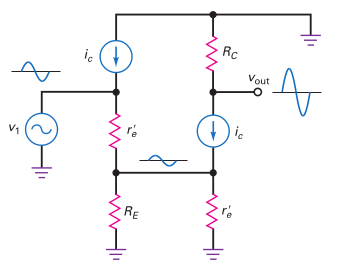
\includegraphics[height=0.7\textheight]{gambar/01.ac_equivalent_circuit}
		\end{center}
		\columnbreak
		\begin{itemize}
			\item Gambar di samping adalah rangkaian ekivalennya
			\item Setiap transistor memiliki $ r'_e $
			\item $ R_E $ paralel dengan $ r'_e $ pada transistor kanan karena base dari $ Q_2 $ di-grounding.
			\item Karena $ R_E $ jauh lebih besar dariada $ r'_e $ maka $ R_E $ bisa diabaikan.
			\item Sehingga kita dapat rangkaian yang lebih sederhana sebagai berikut:
		\end{itemize}
	\end{multicols}
\end{frame}

\begin{frame}{Single-ended output gain}
	\begin{multicols}{2}
		\begin{center}
			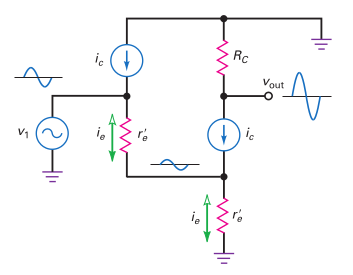
\includegraphics[height=0.7\textheight]{gambar/01.simplified_ac-equivalent_circuit}
		\end{center}
		\columnbreak
		\begin{itemize}
			\item Tegangan input $ v_1 $ sepanjang kedua $ r'_e $
			\item Karena kedua $ r'_e $ bernilai sama, maka tegangan pada $ r'_e $ adalah setengah dari tegangan inputnya.
			\item Ini lah mengapa tegangan AC sepanjang resistor tail adalah setengah dari tegangan input.
		\end{itemize}
	\end{multicols}
\end{frame}

\begin{frame}{Single-ended output gain}
	\begin{multicols}{2}
		\begin{center}
			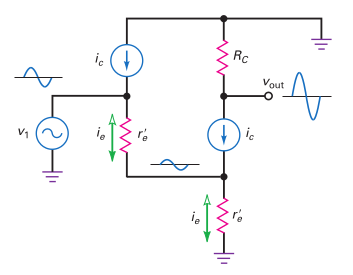
\includegraphics[height=0.7\textheight]{gambar/01.simplified_ac-equivalent_circuit}
		\end{center}
		\columnbreak
		\begin{itemize}
			\item Tegangan output AC: $$ v_{out} = i_C R_C $$
			\item Tegangan input AC: $$ v_{in} = i_e r'_e + i_e r'_e = 2i_er'_e $$
			\item Penguatan tegangan (voltage gain), yaitu $ v_{out} $ dibagi $ v_{in} $, sehingga
			\begin{equation}
				\text{single-ended output: } A_v = \frac{R_C}{2r'_e}
			\end{equation}
		\end{itemize}
	\end{multicols}
\end{frame}

\subsection{Differential-Output Gain}
\begin{frame}{Differential output gain}
	\begin{multicols}{2}
		\begin{center}
			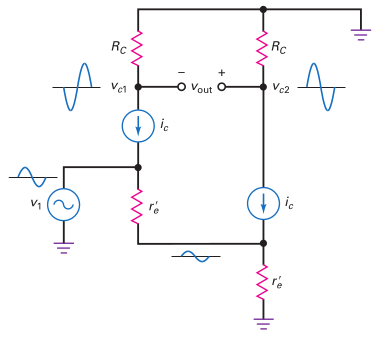
\includegraphics[height=0.7\textheight]{gambar/01.noninverting_input_and_differential_output}
		\end{center}
		\columnbreak
		\begin{itemize}
			\item Gambar di samping adalah rangkaian ekivalen dari noninverting input \& differential output.
			\item Analisis mirip dengan sebelumnya, kecuali tegangan outputnya adalah dua kalinya karena terdapat 2 resistor collector.
			\begin{align*}
				v_{out} &= v_{C2} - v_{C1} = i_C R_C - (-i_C R_C) \\
				&= 2 i_C R_C
			\end{align*}
			\item Tanda negatif $ \rightarrow $ sinyal $ v_{C1} $ memiliki beda fasa sebesar $ \pi $
		\end{itemize}
	\end{multicols}
\end{frame}

\begin{frame}{Differential output gain}
	\begin{multicols}{2}
		\begin{center}
			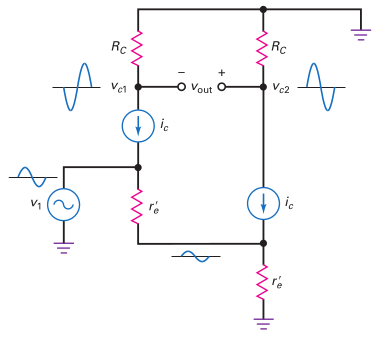
\includegraphics[height=0.7\textheight]{gambar/01.noninverting_input_and_differential_output}
		\end{center}
		\columnbreak
		\begin{itemize}
			\item Tegangan input AC nya masih sama
			\[ v_{in} = 2 i_e r'_e \]
			\item Voltage gain : 
			\begin{equation}
				\text{Differential output }: A_v = \frac{R_C}{r'_e}
			\end{equation}
		\end{itemize}
	\end{multicols}
\end{frame}

\subsection{Konfigurasi inverting-input}
\begin{frame}{Konfigurasi inverting-input}
	\begin{multicols}{2}
		\begin{center}
			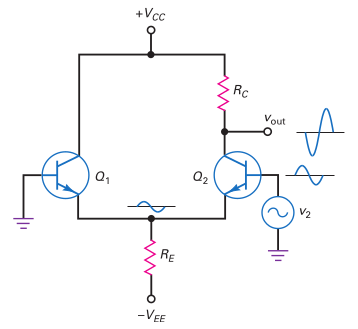
\includegraphics[height=0.7\textheight]{gambar/01.inverting_input_+single-ended_output}
		\end{center}
		\columnbreak
		\begin{itemize}
			\item Gambar di samping adalah inverting input dan single-ended output
			\item Analisis AC hampir sama dengan analisis noninverting
			\item Inverting input $ v_2 $ menghasilkan tegangan output yang diperkuat dan terbalik
			\item $ r'_e $ masih bagian dari pembagi tegangan $ \rightarrow $ tegangan di seberang $ R_E $ setengah dari tegangan inverting input
			\item Jika menggunakan differential output, voltage gainnya adalah bernilai dua kalinya
		\end{itemize}
	\end{multicols}
\end{frame}

\subsection{Konfigurasi differential-input}
\begin{frame}{Konfigurasi differential-input}
	\begin{itemize}
		\item Pada konfigurasi differential-input $ \rightarrow $ kedua inputnya aktif secara bersamaan
		\item Analisis AC dengan menggunakan teorema superposisi
		\item Tegangan output untuk noninverting input adalah $$ v_{out} = A_v(v_1) $$ dan tegangan output untuk inverting input adalah $$ v_{out} = -A_v (v_2) $$
		\item Gabungkan keduanya, $$ v_{out} = A_v (v_1 - v_2) $$
	\end{itemize}
\end{frame}

\subsection{Impedansi Input}
\begin{frame}{Impedansi input}
	\begin{itemize}
		\item Pada CE stage, impedansi input dari base adalah
		\[ z_{in} = \beta r'_e \]
		\item Pada diff amp, impedansi input dari salah satu base adalah dua kalinya
		\begin{equation}
			z_{in} = 2 \beta r'_e
		\end{equation}
		\item Karena terdapat 2 resistor emitter AC $ r'_e $ di dalam rangkaian ekivalennya
	\end{itemize}
\end{frame}

\subsection{Ringkasan}
\begin{frame}{Ringkasan}
	\begin{center}
		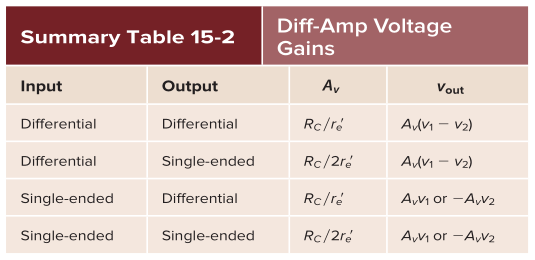
\includegraphics[height=0.7\textheight]{gambar/01.summary-diff-amp_voltage_gains}
	\end{center}
\end{frame}

\subsection{Contoh Soal 1.4}
\begin{frame}{Contoh Soal 1.4}
	\begin{multicols}{2}
		\begin{center}
			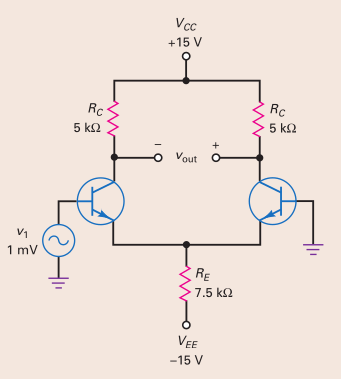
\includegraphics[height=0.7\textheight]{gambar/01.contoh_soal_1-2}
		\end{center}
		\columnbreak
		\begin{itemize}
			\item Pertanyaan:
			\begin{itemize}
				\item Berdasarkan gambar di samping, berapa tegangan output AC? Jika $ \beta = 300 $, berapa impedansi input dari diff amp tersebut ?
			\end{itemize}
		\end{itemize}
	\end{multicols}
\end{frame}

\begin{frame}{Contoh Soal 1.4}
	\begin{multicols}{2}
		\begin{center}
			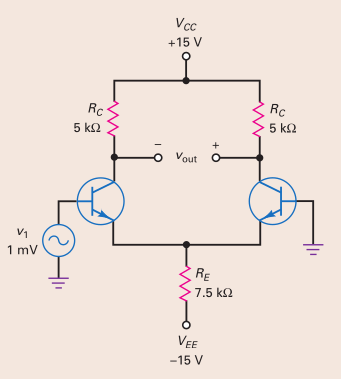
\includegraphics[height=0.7\textheight]{gambar/01.contoh_soal_1-2}
		\end{center}
		\columnbreak
		\begin{itemize}
			\item Jawaban:
			\begin{itemize}
				\item Idealnya, 15 V di seberang resistor emitter, menghasilkan arus tail sebesar 2 mA, yang artinya arus emitter DC pada masing masing transistor sebesar
				\[ I_E = 1 \text{ mA} \]
				\item Lalu kita hitung resistansi emitternya
				\[ r'_e = \frac{25 \text{ mV}}{ I_E} =\frac{25 \text{ mV}}{1 \text{ mA}} = 25~\Omega \]
			\end{itemize}
		\end{itemize}
	\end{multicols}
\end{frame}

\begin{frame}{Contoh Soal 1.4}
	\begin{multicols}{2}
		\begin{center}
			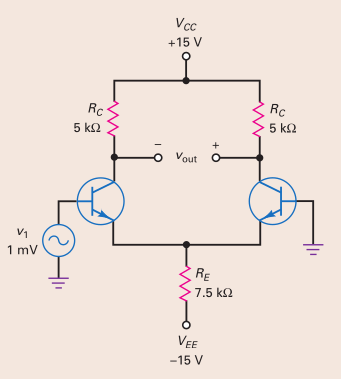
\includegraphics[height=0.7\textheight]{gambar/01.contoh_soal_1-2}
		\end{center}
		\columnbreak
		\begin{itemize}
			\item Jawaban:
			\begin{itemize}
				\item Voltage gain:
				\[ A_v = \frac{R_C}{r'_e} = \frac{5 \text{ k}\Omega }{25 \text{ }\Omega } = 200 \]
				\item Tegangan keluaran AC
				\[ v_{out} = A_v v_1 = 200(1 \text{ mV}) = 200 \text{ mV} \]
				\item Impedansi input
				\[ z_{in(base)} = 2 \beta r'_e = 2(300)(25\Omega) = 15 \text{ k}\Omega\]
			\end{itemize}
		\end{itemize}
	\end{multicols}
\end{frame}

\subsection{Latihan Soal 1.4}
\begin{frame}{Latihan Soal 1.4}
	\begin{multicols}{2}
		\begin{center}
			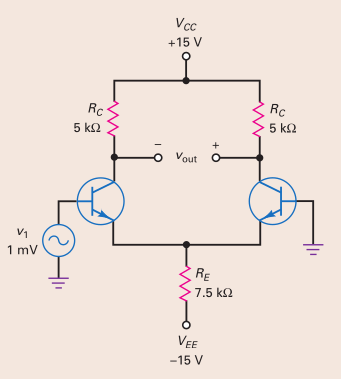
\includegraphics[height=0.7\textheight]{gambar/01.contoh_soal_1-2}
		\end{center}
		\columnbreak
		\begin{itemize}
			\item Pertanyaan:
			\begin{itemize}
				\item Berdasarkan gambar di samping, jika $ R_E = 5 \text{ k}\Omega $, berapa tegangan output AC? Jika $ \beta = 300 $, berapa impedansi input dari diff amp tersebut ?
			\end{itemize}
			\item Jawaban:
			\begin{itemize}
				\item Silakan dikerjakan
			\end{itemize}
		\end{itemize}
	\end{multicols}
\end{frame}

\subsection{Contoh Soal 1.5}
\begin{frame}{Contoh Soal 1.5}
	\begin{multicols}{2}
		\begin{center}
			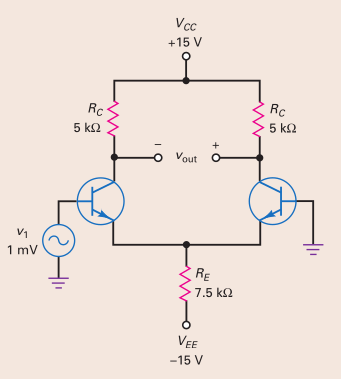
\includegraphics[height=0.7\textheight]{gambar/01.contoh_soal_1-2}
		\end{center}
		\columnbreak
		\begin{itemize}
			\item Pertanyaan:
			\begin{itemize}
				\item Berdasarkan gambar di samping, jika menggunakan metode ke 2, berapa tegangan output AC? Jika $ \beta = 300 $, berapa impedansi input dari diff amp tersebut ?
			\end{itemize}
		\end{itemize}
	\end{multicols}
\end{frame}

\begin{frame}{Contoh Soal 1.5}
	\begin{multicols}{2}
		\begin{center}
			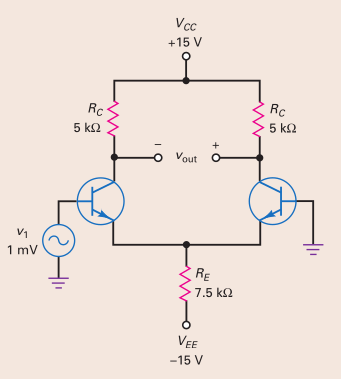
\includegraphics[height=0.7\textheight]{gambar/01.contoh_soal_1-2}
		\end{center}
		\columnbreak
		\begin{itemize}
			\item Jawaban:
			\begin{itemize}
				\item Tentukan arus tail
				\begin{align*}
					I_T &= \frac{V_{EE} - V_{BE}}{R_E} = \frac{15 \text{ V} - 0.7 \text{ V}}{7.5 \text{ k}\Omega} \\
					&= 1.91 \text{ mA}
				\end{align*}
				\item Arus emitter DC
				\[ I_E = \frac{I_T}{2} = \frac{1.91}{2} = 0.955 \text{ mA}\]
				\item Resistansi emitter AC
				\[ r'_e = \frac{25 \text{ mV}}{ I_E} =\frac{25 \text{ mV}}{0.955 \text{ mA}} = 26.2~\Omega \]
			\end{itemize}
		\end{itemize}
	\end{multicols}
\end{frame}

\begin{frame}{Contoh Soal 1.5}
	\begin{multicols}{2}
		\begin{center}
			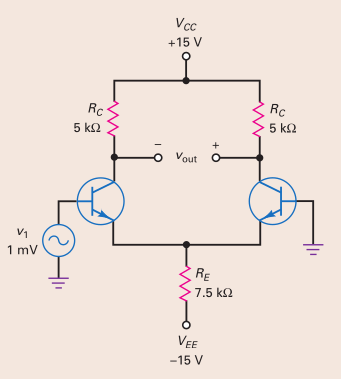
\includegraphics[height=0.7\textheight]{gambar/01.contoh_soal_1-2}
		\end{center}
		\columnbreak
		\begin{itemize}
			\item Jawaban:
			\begin{itemize}
				\item Voltage gain
				\[ A_v = \frac{R_C}{r'_e} = \frac{5 \text{ k}\Omega }{26.2 \text{ }\Omega } = 191 \]
				\item Tegangan keluaran AC
				\[ v_{out} = A_v v_1 = 191(1 \text{ mV}) = 191 \text{ mV} \]
				\item Impedansi input
				\[ z_{in(base)} = 2 \beta r'_e = 2(300)(26.2\Omega) = 15.7 \text{ k}\Omega\]
			\end{itemize}
		\end{itemize}
	\end{multicols}
\end{frame}

\subsection{Contoh Soal 1.6}
\begin{frame}{Contoh Soal 1.6}
	\begin{multicols}{2}
		\begin{center}
			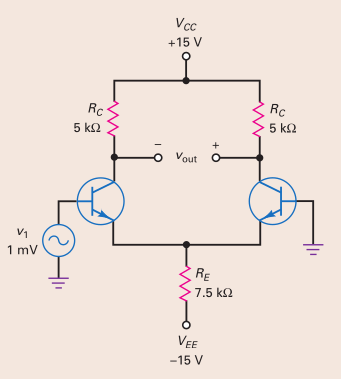
\includegraphics[height=0.7\textheight]{gambar/01.contoh_soal_1-2}
		\end{center}
		\columnbreak
		\begin{itemize}
			\item Pertanyaan:
			\begin{itemize}
				\item Jika pada gambar di samping $ v_2 = 1 \text{ mV} $ dan $ v_1 = 0 $ maka berapa tegangan output AC? Jika $ \beta = 300 $, maka berapa impedansi inputnya?
			\end{itemize}
			\item Jawaban:
			\begin{itemize}
				\item Hasilnya sama dengan Contoh Soal 1.4, hanya saja memiliki magnitude yang berkebalikan karena menggunakan inverting input.
			\end{itemize}
		\end{itemize}
	\end{multicols}
\end{frame}

\subsection{Contoh Soal 1.7}
\begin{frame}{Contoh Soal 1.7}
	\begin{multicols}{2}
		\begin{center}
			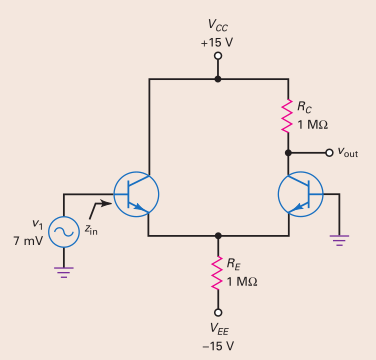
\includegraphics[height=0.7\textheight]{gambar/01.contoh_soal_07}
		\end{center}
		\columnbreak
		\begin{itemize}
			\item Pertanyaan:
			\begin{itemize}
				\item Berdasarkan gambar di samping, jika $ \beta = 300 $, berapa impedansi input dari diff amp tersebut ?
			\end{itemize}
		\end{itemize}
	\end{multicols}
\end{frame}

\begin{frame}{Contoh Soal 1.7}
	\begin{multicols}{2}
		\begin{center}
			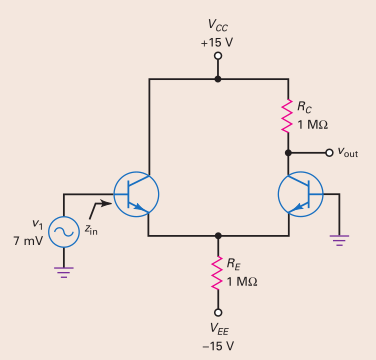
\includegraphics[height=0.7\textheight]{gambar/01.contoh_soal_07}
		\end{center}
		\columnbreak
		\begin{itemize}
			\item Jawaban:
			\begin{itemize}
				\item Idealnya sebesar 15 V pada emitter resistor, sehingga arus tailnya:
				\[ I_T = \frac{V_{EE}}{R_E} = \frac{15 \text{ V}}{1 \text{ M}\Omega} = 15~\mu\text{A} \]
				\item Karena arus emitter di setiap transistornya adalah separuh dari arus tail, maka resistansi dari emitternya adalah:
				\[ r'_e = \frac{25 \text{ mV}}{ I_E} =\frac{25 \text{ mV}}{7.5 \mu\text{ A}} = 3.33 \text{ k}\Omega \]
			\end{itemize}
		\end{itemize}
	\end{multicols}
\end{frame}

\begin{frame}{Contoh Soal 1.7}
	\begin{multicols}{2}
		\begin{center}
			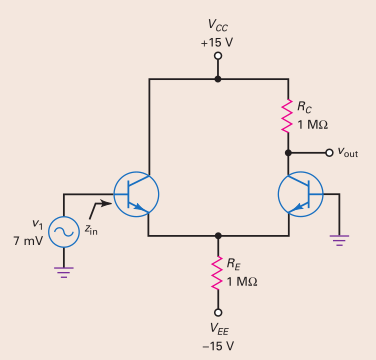
\includegraphics[height=0.7\textheight]{gambar/01.contoh_soal_07}
		\end{center}
		\columnbreak
		\begin{itemize}
			\item Jawaban:
			\begin{itemize}
				\item Voltage gain
				\[ A_v = \frac{R_C}{2r'_e} = \frac{1 \text{ M}\Omega }{2 (3.33 \text{ k}\Omega) } = 150 \]
				\item Tegangan keluaran AC
				\[ v_{out} = A_v v_1 = 150(7 \text{ mV}) = 1.05 \text{ V} \]
				\item Impedansi input
				\begin{align*}
					z_{in(base)} &= 2 \beta r'_e = 2(300)(3.33 \text{ k}\Omega) \\
					&= 2 \text{ M}\Omega
				\end{align*}
			\end{itemize}
		\end{itemize}
	\end{multicols}
\end{frame}

\subsection{Latihan Soal 1.7}
\begin{frame}{Latihan Soal 1.7}
	\begin{multicols}{2}
		\begin{center}
			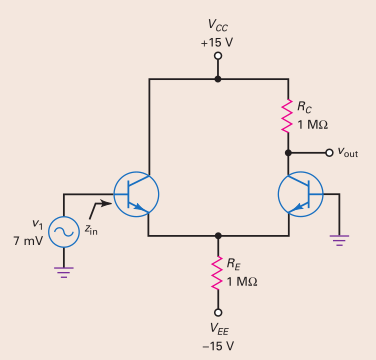
\includegraphics[height=0.7\textheight]{gambar/01.contoh_soal_07}
		\end{center}
		\columnbreak
		\begin{itemize}
			\item Pertanyaan:
			\begin{itemize}
				\item Berdasarkan gambar di samping, jika $ \beta = 300 $ dan $ R_E = 500 \text{ k}\Omega $, berapa impedansi input dari diff amp tersebut ?
			\end{itemize}
		\end{itemize}
	\end{multicols}
\end{frame}


\section{Karakteristik Input dari Sebuah Op Amp}
\begin{frame}{Karakteristik Input dari Sebuah Op Amp}
	\begin{itemize}
		\item Asumsi bahwa diff amp simetris (transistor yang digunakan identik) adalah metode pendekatan yang bagus untuk beberapa aplikasi.
		\item Namun pada aplikasi yang lebih presisi, kita tidak bisa lagi mengasumsikan bahwa keduanya identik.
		\item Terdapat 3 karakteristik pada datasheet setiap op amp yang biasanya digunakan oleh para engineer yang membutuhkan akurasi yg tinggi.
		\item Karakteristik tersebut antara lain:
		\begin{enumerate}
			\item Arus bias input
			\item Arus offset input
			\item Tegangan offset input
		\end{enumerate}
	\end{itemize}
\end{frame}

\subsection{Arus Bias Input}
\begin{frame}{Arus bias input}
	\begin{multicols}{2}
		\begin{center}
			\includegraphics[height=0.7\textheight]{gambar/01.different_base_currents}
		\end{center}
		\columnbreak
		\begin{itemize}
			\item Pada op amp yang terintegrasi, $ \beta_{dc} $ dari masing-masing transistor pada stage yang pertama sedikit berbeda
			\item Sehingga arus base juga sedikit berbeda, seperti yang ditampilkan pada gambar di samping.
			\item Arus bias input didefinisikan sebagai rata-rata dari arus base DC:
			\begin{equation}
				I_{in(bias)} = \frac{I_{B1} + I_{B2}}{2}
			\end{equation}
		\end{itemize}
	\end{multicols}
\end{frame}

\begin{frame}{Arus bias input}
	\begin{multicols}{2}
		\begin{center}
			\includegraphics[height=0.7\textheight]{gambar/01.different_base_currents}
		\end{center}
		\columnbreak
		\begin{itemize}
			\item Misalkan, jika $ I_{B1} = 90 \text{ nA} $ dan $ I_{B2} = 70 \text{ nA} $, maka arus bias input-nya adalah:
			\[ I_{in(bias)} = \frac{ 90 \text{ nA} + 70 \text{ nA} }{2} = 80 \text{ nA}\]
			\item Jika menggunakan BJT, biasanya arus bias input sebesar $ \text{ nA} $. Jika menggunakan JFET, biasanya arus bias inputnya sebesar $ \text{ pA} $.
		\end{itemize}
	\end{multicols}
\end{frame}

\subsection{Arus Offset Input}
\begin{frame}{Arus offset input}
	\begin{itemize}
		\item Arus offset input didefinisikan sebagai perbedaan arus base DC
		\begin{equation}
			I_{in(off)} = I_{B1} - I_{B2}
		\end{equation}
		\item Perbedaan di dalam arus base mengindikasikan seberapa mirip transistornya.
		\item Jika transistornya identik, arus offset inputnya akan bernilai nol.
		\item Tapi, kedua transistor hampir selalu berbeda dan kedua arus basenya tidak sama.
		\item Misalkan, jika $ I_{B1} = 90 \text{ nA} $ dan $ I_{B2} = 70 \text{ nA} $, maka arus offset input-nya adalah:
		\[ I_{in(off)} = 90 \text{ nA} - 70 \text{ nA} = 20 \text{ nA}\]
		\item Artinya, transistor $ Q_1 $ memiliki lebih 20 nA arus base dari pada transistor $ Q_2 $. Hal ini akan menyebabkan masalah nantinya ketika menggunakan resistansi base yang besar.
	\end{itemize}
\end{frame}

\subsection{Arus Base dan Offset}
\begin{frame}{Arus base dan offset}
	\begin{itemize}
		\item Kita bisa turunkan persamaan arus bias dan arus offset input menjadi:
		\begin{align*}
			I_{B1} &= I_{in(bias)} + \frac{I_{in(off)}}{2} \tag{13.a} \label{13.a}\\
			I_{B2} &= I_{in(bias)} - \frac{I_{in(off)}}{2}	\tag{13.b} \label{13.b}
		\end{align*}
		\item Datasheet hanya menunjukkan $ I_{in(bias)} $ dan $ I_{in(off)} $, bukan $ I_{B1} $ dan $ I_{B2} $. Sehingga dengan persamaan \ref{13.a} \& \ref{13.b}, kita dapat menghitung arus base-nya.
		\item Persamaan \ref{13.a} \& \ref{13.b} mengasumsikan bahwa $ I_{B1} > I_{B2} $. Jika $ I_{B1} < I_{B2} $, maka ubah urutan persamaannya.
	\end{itemize}
\end{frame}

\subsection{Pengaruh dari Arus Base}
\begin{frame}{Pengaruh dari Arus Base}
	\begin{multicols}{2}
		\begin{center}
			\includegraphics[height=0.7\textheight]{gambar/01.base_resistor_produces_unwanted_input_voltage}
		\end{center}
		\begin{itemize}
			\item Beberapa diff amp beroperasi dengan sebuah resistor base di satu sisi saja.
			\item Karena arah arus base, arus base melalui $ R_B $ menghasilkan tegangan input dc noninverting sebesar
			\[ V_1 = -I_{B1}R_B \]
			\item Resistor base menghasilkan tegangan input yang tidak diinginkan
			\item \textbf{Catatan:} Huruf kapital menunjukkan tegangan error dc ($ V_1 $) dan kita gunakan nilai absolut
		\end{itemize}
	\end{multicols}
\end{frame}

\begin{frame}{Pengaruh dari Arus Base}
	\begin{multicols}{2}
		\begin{center}
			\includegraphics[height=0.7\textheight]{gambar/01.base_resistor_produces_unwanted_input_voltage}
		\end{center}
	\columnbreak
		\begin{itemize}
			\item Sebagai contoh, jika di datasheet $ I_{in(bias)} = 80 \text{ nA} $ dan $ I_{in(off)} = 20 \text{ nA}$, maka
			\begin{align*}
				I_{B1} &= I_{in(bias)} + \frac{I_{in(off)}}{2} \\
				&= 80 \text{ nA} + \frac{20 \text{ nA}}{2} = 90 \text{ nA} \\
				I_{B2} &= I_{in(bias)} - \frac{I_{in(off)}}{2} \\
				&= 80 \text{ nA} - \frac{20 \text{ nA}}{2} = 70 \text{ nA}
			\end{align*}
		\end{itemize}
	\end{multicols}
\end{frame}

\begin{frame}{Pengaruh dari Arus Base}
	\begin{multicols}{2}
		\begin{center}
			\includegraphics[height=0.7\textheight]{gambar/01.base_resistor_produces_unwanted_input_voltage}
		\end{center}
		\columnbreak
		\begin{itemize}
			\item Jika $ R_B = 1 \text{ k}\Omega $, input noninverting memiliki error tegangan sebesar
			\begin{align*}
				V_1 &= -I_{B1}R_B \\
				&= ( 90 \text{ nA} ) ( 1 \text{ k}\Omega ) \\
				&= 90 \text{ }\mu V
			\end{align*}
		\end{itemize}
	\end{multicols}
\end{frame}

\subsection{Pengaruh dari Arus Offset Input}
\begin{frame}{Pengaruh dari Arus Offset Input}
	\begin{multicols}{2}
		\begin{center}
			\includegraphics[height=0.7\textheight]{gambar/01.equal_base_resistance_on_other_side_reduces_error}
		\end{center}
		\columnbreak
		\begin{itemize}
			\item Cara mengurangi error tegangan output dengan menggunakan resistor base yang sama pada sisi lainnya, seperti gambar di samping.
			\item Sehingga kita memiliki differential dc input
			\begin{align*}
				V_{in} &= I_{B1}R_B - I_{B2}R_B \\
				&= (I_{B1} - I_{B2})R_B				
			\end{align*}
			\begin{equation}
				V_{in} = I_{in(off)}R_B
			\end{equation}
		\end{itemize}
	\end{multicols}
\end{frame}

\begin{frame}{Pengaruh dari Arus Offset Input}
	\begin{multicols}{2}
		\begin{center}
			\includegraphics[height=0.7\textheight]{gambar/01.equal_base_resistance_on_other_side_reduces_error}
		\end{center}
		\columnbreak
		\begin{itemize}
			\item Karena biasanya $ I_{in(off)}  < (0.25)( I_{in(bias)})$, error tegangan input jauh lebih kecil ketika resistor base yang sama digunakan.
			\item Sebagai contoh, jika $ I_{in(bias)} = 80 \text{ nA} $ dan $ I_{in(off)} = 20 \text{ nA} $, lalu resistor base sebesar $ 1 \text{ k}\Omega $ menghasilkan error tegangan input sebesar
			\begin{align*}
				V_{in} &= (I_{in(off)})(R_B) \\
				&= (20 \text{ nA})(1 \text{ k}\Omega) = 20 \text{ }\mu\text{V}\\
			\end{align*}
		\end{itemize}
	\end{multicols}
\end{frame}

\subsection{Tegangan Offset Input}
\begin{frame}{Tegangan Offset Input}
	\begin{multicols}{2}
		\begin{center}
			\includegraphics[height=0.7\textheight]{gambar/01.different_collector_resistors_produce_error_when_bases_are_grounded}
		\end{center}
		\columnbreak
		\begin{itemize}
			\item Ketika diff amp terintegrasi sebagai first stage dari op amp, kedua sisinya hampir identik
			\item Kedua resistor collector bisa saja berbeda
			\item Akibatnya muncul error tegangan di output-nya
		\end{itemize}
	\end{multicols}
\end{frame}

\begin{frame}{Tegangan Offset Input}
	\begin{multicols}{2}
		\begin{center}
			\includegraphics[height=0.7\textheight]{gambar/01.different_base-emitter_curves_added_to_error}
		\end{center}
		\columnbreak
		\begin{itemize}
			\item Sumber error lainnya adalah perbedaan kurva $ V_{BE} $ dari transistornya
			\item Sebagai contoh, anggaplah kedua kurva base-emitter memiliki arus yang sama seperti gambar di samping
			\item Karena kurva tersebut berbeda, maka terdapat perbedaan antara kedua $ V_{BE} $
			\item Perbedaan ini menyebabkan penambahan error tegangan
		\end{itemize}
	\end{multicols}
\end{frame}

\begin{frame}{Tegangan Offset Input}
	\begin{multicols}{2}
		\begin{center}
			\includegraphics[height=0.4\textheight]{gambar/01.input_offset_voltage_is_equivalent_to_an_unwanted_input_voltage}
		\end{center}
		\columnbreak
		\begin{itemize}
			\item Tegangan offset input = tegangan input yang menghasilkan error tegangan ouput yang sama di diff amp yang ideal
			\begin{equation}
				V_{in(off)} = \frac{V_{error}}{A_v}
			\end{equation}
			\item $ V_{error} $ tidak menyertakan efek bias input dan arus offset karena kedua base di-ground ketika $ V_{error} $ diukur.
		\end{itemize}
	\end{multicols}
\end{frame}

\begin{frame}{Tegangan Offset Input}
	\begin{multicols}{2}
		\begin{center}
			\includegraphics[height=0.4\textheight]{gambar/01.input_offset_voltage_is_equivalent_to_an_unwanted_input_voltage}
		\end{center}
		\columnbreak
		\begin{itemize}
			\item Sebagai contoh, jika diff amp memiliki error tegangan sebesar $ 0.6 \text{ V} $ dan penguatan tegangan sebesar 300, tegangan offset input adalah
			\begin{align*}
				V_{in(off)} = \frac{V_{error}}{A_v} = \frac{0.6 \text{ V}}{300} = 2 \text{ mV}
			\end{align*}
			\item Gambar di samping mengilustrasikan tegangan offset input sebesar $ 2 \text{ mV} $ menghasilkan error tegangan sebesar $ 0.6 \text{ V} $
		\end{itemize}
	\end{multicols}
\end{frame}

\subsection{Efek Gabungan}
\begin{frame}{Efek Gabungan}
	\begin{multicols}{2}
		\begin{figure}
			\centering
			\includegraphics[height=0.6\textheight]{gambar/01.output_of_diff_amp_includes_desired_signal_and_error_voltage}
		\end{figure}
		\columnbreak
		\begin{itemize}
			\item Tegangan output adalah superposisi dari semua efek input
			\item Terdapat input ac ideal: $$ v_{in} = v_1 - v_2 $$
			\item Dari 2 sumber input, dikuatkan, menghasilkan output ac yang diinginkan: $$ v_{out} = A_v(v_1 - v_2) $$
		\end{itemize}
	\end{multicols}
\end{frame}

\begin{frame}{Efek Gabungan}
	\begin{multicols}{2}
		\begin{figure}
			\centering
			\includegraphics[height=0.6\textheight]{gambar/01.output_of_diff_amp_includes_desired_signal_and_error_voltage}
		\end{figure}
		\columnbreak
		\begin{itemize}
			\item Terdapat 3 error input dc:
			\begin{equation}
				V_{1err} = (R_{B1} - R_{B2}) I_{in(bias)}
			\end{equation}
			\begin{equation}
				V_{2err} = (R_{B1} + R_{B2}) \frac{I_{in(off)}}{2}
			\end{equation}
			\begin{equation}
				V_{3err} = V_{in(off)}
			\end{equation}
			\item Ketiga error dc dikuatkan kemudian menghasilkan error tegangan output:
			\begin{equation}
				V_{error} = A_v (V_{1err} + V_{2err} + V_{3err})
			\end{equation}
		\end{itemize}
	\end{multicols}
\end{frame}

\begin{frame}{Efek Gabungan}
	\begin{multicols}{2}
		\begin{figure}
			\centering
			\includegraphics[height=0.6\textheight]{gambar/01.output_of_diff_amp_includes_desired_signal_and_error_voltage}
		\end{figure}
		\columnbreak
		\begin{itemize}
			\item Dalam aplikasinya, $ V_{error} $ dapat diabaikan. Misalnya kita akan membuat ac amplifier, $ V_{error} $ tidak lah penting. Kecuali kita akan membuat dc amplifier yang presisi, maka $ V_{error} $ perlu diperhatikan.
		\end{itemize}
	\end{multicols}
\end{frame}

\subsection{Resistor Base yang Sama}
\begin{frame}{Resistor Base yang Sama}
	\begin{itemize}
		\item Ketika error offset dan bias tidak dapat diabaikan, maka hal yang bisa dilakukan adalah gunakan resistor base yang sama: $ R_{B1} = R_{B2} = R_{B}$
		\item Karena:
		\begin{align*}
			V_{1err} &= 0 \\
			V_{2err} &= R_B I_{in(off)} \\
			V_{3err} &= V_{in(off)}
		\end{align*}
		\item Atau bisa menggunakan rangkaian nulling yang tersedia di datasheet $ \leftarrow $ akan dijelaskan pada bab selanjutnya.
	\end{itemize}
\end{frame}

\subsection{Ringkasan}
\begin{frame}{Ringkasan}
	\begin{center}
		\includegraphics[height=0.7\textheight]{gambar/01.ringkasan_3}
	\end{center}
\end{frame}

\subsection{Contoh Soal 1.8}
\begin{frame}{Contoh Soal 1.8}
	\begin{multicols}{2}
		\begin{center}
			\includegraphics[height=0.7\textheight]{gambar/01.latihan_soal_8}
		\end{center}
		\columnbreak
		\begin{itemize}
			\item Pertanyaan:
			\begin{itemize}
				\item Diff amp di samping memiliki $ A_v = 200 $,\\ $ I_{in(bias)} = 3~\mu\text{A} $, \\ $ I_{in(off)} = 0.5~\mu\text{A} $, \\ $ V_{in(off)} = 1 \text{ mV}$.  
				\item Berapa error tegangan output?
				\item Jika menggunakan resistor base yang identik, berapa error tegangan output?
			\end{itemize}
		\end{itemize}
	\end{multicols}
\end{frame}

\begin{frame}{Contoh Soal 1.8}
	\begin{multicols}{2}
		\begin{center}
			\includegraphics[height=0.7\textheight]{gambar/01.latihan_soal_8}
		\end{center}
		\columnbreak
		\begin{itemize}
			\item Jawaban:
			\begin{itemize}
				\item Masing-masing error tegangan:
				\begin{align*}
					V_{1err} &= (R_{B1} - R_{B2}) I_{in(bias)} \\
					&= (1 \text{ k}\Omega)(3~\mu\text{A}) = 3 \text{ mV} \\
					V_{2err} &= (R_{B1} + R_{B2}) \frac{I_{in(off)}}{2} \\
					&= (1 \text{ k}\Omega)(0.25~\mu\text{A}) = 0.25 \text{ mV} \\
					V_{3err} &= V_{in(off)} = 1 \text{ mV}
				\end{align*}
			\end{itemize}
		\end{itemize}
	\end{multicols}
\end{frame}

\begin{frame}{Contoh Soal 1.8}
	\begin{multicols}{2}
		\begin{center}
			\includegraphics[height=0.7\textheight]{gambar/01.latihan_soal_8}
		\end{center}
		\columnbreak
		\begin{itemize}
			\item Jawaban:
			\begin{itemize}
				\item Error tegangan output:
				\begin{align*}
					V_{error} &= A_v (V_{1err} + V_{2err} + V_{3err}) \\
					&= 200(3 \text{ mV} + 0.25 \text{ mV} + 1 \text{ mV}) \\
					&= 850 \text{ mV}
				\end{align*}
			\end{itemize}
			\begin{itemize}
				\item Jika menggunakan resistor base yang identik di bagian inverting input:
				\begin{align*}
					V_{1err} &= 0 \\
					V_{2err} &= R_{B}I_{in(off)} \\
					&= (1 \text{ k}\Omega)(0.5~\mu\text{A}) = 0.5 \text{ mV} \\
					V_{3err} &= V_{in(off)} = 1 \text{ mV}
				\end{align*}
			\end{itemize}
		\end{itemize}
	\end{multicols}
\end{frame}

\begin{frame}{Contoh Soal 1.8}
	\begin{multicols}{2}
		\begin{center}
			\includegraphics[height=0.7\textheight]{gambar/01.latihan_soal_8}
		\end{center}
		\columnbreak
		\begin{itemize}
			\item Jawaban:
			\begin{itemize}
				\item Error tegangan output:
				\begin{align*}
					V_{error} &= A_v (V_{1err} + V_{2err} + V_{3err}) \\
					&= 200(0.5 \text{ mV} + 1 \text{ mV}) \\
					&= 300 \text{ mV}
				\end{align*}
			\end{itemize}
		\end{itemize}
	\end{multicols}
\end{frame}

\subsection{Latihan Soal 1.8}
\begin{frame}{Latihan Soal 1.8}
	\begin{multicols}{2}
		\begin{center}
			\includegraphics[height=0.7\textheight]{gambar/01.latihan_soal_8}
		\end{center}
		\columnbreak
		\begin{itemize}
			\item Pertanyaan:
			\begin{itemize}
				\item Berapa error tegangan output jika diff amp tersebut memiliki penguatan tegangan sebesar 150?
			\end{itemize}
			\item Jawaban: \textit{Silakan dikerjakan}
		\end{itemize}
	\end{multicols}
\end{frame}

\subsection{Contoh Soal 1.9}
\begin{frame}{Contoh Soal 1.9}
	\begin{multicols}{2}
		\begin{center}
			\includegraphics[height=0.7\textheight]{gambar/01.contoh_soal_9}
		\end{center}
		\columnbreak
		\begin{itemize}
			\item Pertanyaan:
			\begin{itemize}
				\item Diketahui diff amp memiliki\\
				$ A_v = 300 $, \\
				$ I_{in(bias)} = 80 \text{ nA}$, \\
				$ I_{in(off)} = 20 \text{ nA}$, dan \\
				$ V_{in(off)} = 5 \text{ mV}$.
				\item Berapa error tegangan output?
			\end{itemize}
		\end{itemize}
	\end{multicols}
\end{frame}

\begin{frame}{Contoh Soal 1.9}
	\begin{multicols}{2}
		\begin{center}
			\includegraphics[height=0.7\textheight]{gambar/01.contoh_soal_9}
		\end{center}
		\columnbreak
		\begin{itemize}
			\item Jawaban:
			\begin{itemize}
				\item Rangkaian tersebut menggunakan resistor base yang sama, maka:
				\begin{align*}
					V_{1err} &= 0 \\
					V_{2err} &= R_{B}I_{in(off)} \\
					&= (10 \text{ k}\Omega)(20 \text{ nA}) = 0.2 \text{ mV} \\
					V_{3err} &= V_{in(off)} = 5 \text{ mV}
				\end{align*}
			\item Total error tegangan output:
			\begin{align*}
				V_{error} &= A_v (V_{1err} + V_{2err} + V_{3err}) \\
				&= 300 (0.2 \text{ mV} + 5 \text{ mV}) \\
				V_{error} &= 1.56 \text{ V}
			\end{align*}
			\end{itemize}
		\end{itemize}
	\end{multicols}
\end{frame}

\subsection{latihan Soal 1.9}
\begin{frame}{Latihan Soal 1.9}
	\begin{multicols}{2}
		\begin{center}
			\includegraphics[height=0.7\textheight]{gambar/01.contoh_soal_9}
		\end{center}
		\columnbreak
		\begin{itemize}
			\item Pertanyaan:
			\begin{itemize}
				\item Diketahui diff amp memiliki\\
				$ A_v = 300 $, \\
				$ I_{in(bias)} = 80 \text{ nA}$, \\
				$ I_{in(off)} = 10 \text{ nA}$, dan \\
				$ V_{in(off)} = 5 \text{ mV}$.
				\item Berapa error tegangan output?
			\end{itemize}
			\item Jawaban: \textit{Silakan dikerjakan}
		\end{itemize}
	\end{multicols}
\end{frame}

\section{Common-Mode Gain}
\subsection{Common-Mode Signal}
\begin{frame}{Common-Mode Signal}
	\begin{multicols}{2}
		\begin{center}
			\includegraphics[height=0.7\textheight]{gambar/01.common-mode_input_signal}
		\end{center}
		\columnbreak
		\begin{itemize}
			\item Rangkaian differential input dan single-ended output
			\item Tegangan input yang sama $( v_{in(CM)} )$ di setiap base $ \rightarrow $ \textbf{common-mode signal}
			\item Jika diff amp benar-benar simetris $ \rightarrow $ tidak ada tegangan output ac dengan common-mode signal karena $ v_1 = v_2 $
			\item Jika diff amp tidak simetris $ \rightarrow $ ada tegangan output ac yang kecil
			\item Jika $ v_1 = v_2 $ maka $ v_{out} = 0 $, lalu untuk apa?
		\end{itemize}
	\end{multicols}
\end{frame}

\begin{frame}{Common-Mode Signal}
	\begin{multicols}{2}
		\begin{center}
			\includegraphics[height=0.7\textheight]{gambar/01.common-mode_input_signal}
		\end{center}
		\columnbreak
		\begin{itemize}
			\item Sebagian besar noise static atau interference = common-mode signal
			\item Bagaimana common-mode signal bisa muncul? $ \rightarrow $ Wiring pada base mirip antena kecil.
			\item Lingkungannya dif amp banyak gelombang elektromagnetik $ \rightarrow $ tiap base akan mengambil sinyal tegangan yang tidak diinginkan
			\item Alasan utama menggunakan diff amp sebagai first stage dari op amp $ \rightarrow $ diff amp tidak menguatkan common-mode signal
		\end{itemize}
	\end{multicols}
\end{frame}

\begin{frame}{Common-Mode Signal}
	\begin{multicols}{2}
		\begin{center}
			\includegraphics[height=0.7\textheight]{gambar/01.equivalent_circuit_commonmode}
		\end{center}
		\columnbreak
		\begin{itemize}
			\item Karena kedua tegangan $ v_{in(CM)} $ sama maka hampir tidak ada arus yang mengalir antara kedua emitter.
			\item Sehingga rangkaian di samping menjadi sebagai berikut ini (slide selanjutnya)
		\end{itemize}
	\end{multicols}
\end{frame}

\subsection{Common-Mode Gain}
\begin{frame}{Common-Mode Gain}
	\begin{multicols}{2}
		\begin{center}
			\includegraphics[height=0.7\textheight]{gambar/01.fig20}
		\end{center}
		\columnbreak
		\begin{itemize}
			\item Dengan common-mode signal, rangkaian bagian kanan ekivalen dengan heavily swamped CE amplifier
			\item Karena $ R_E $ jauh lebih besar daripada $ r'_e $, swamped voltage gain (penguatan tegangan terbenam) adalah
			\begin{equation}\label{pers.20}
				A_{v(CM)} = \frac{R_C}{2R_E}
			\end{equation}
			\item Biasanya $ A_{v(CM)} < 1 $
		\end{itemize}
	\end{multicols}
\end{frame}

\subsection{Common-Mode Rejection Ratio (CMRR)}
\begin{frame}{Common-Mode Rejection Ratio (CMRR)}
	\begin{itemize}
		\item Common-Mode Rejection Ratio (CMRR) :
		\begin{equation}\label{pers.21}
			\text{CMMR} = \frac{A_v}{A_{v(CM)}}
		\end{equation}
		\item Misalkan $ A_v = 200 $ dan $ A_{v(CM)} = 0.5 $ maka CMMR = 400
		\item Semakin tinggi nilai CMRR, maka semakin baik.
		\item CMRR yang tinggi : menaikkan sinyal yang diinginkan dan tidak untuk common-mode signal-nya
		\item Datasheet biasanya menampilkan CMRR dalam satuan decibels (dB)
		\begin{equation}\label{pers.22}
			\text{CMRR}_{dB} = 20 \log \text{CMRR}
		\end{equation}
		\item Misalkan CMRR = 400 maka $ \text{CMRR}_{dB} = 52 \text{ dB} $
	\end{itemize}
\end{frame}

\subsection{Contoh Soal 1.10}
\begin{frame}{Contoh Soal 1.10}
	\begin{multicols}{2}
		\begin{center}
			\includegraphics[height=0.7\textheight]{gambar/01.fig21}
		\end{center}
		\columnbreak
		\begin{itemize}
			\item Pertanyaan:
			\begin{itemize}
				\item Berapa common-mode voltage gain?
				\item Berapa tegangan output?
			\end{itemize}
			\item Jawaban:
			\begin{itemize}
				\item $ A_{v(CM)} = \frac{R_C}{2R_E} = \frac{1 \text{ M}\Omega}{1 \text{ M}\Omega} = 0.5 $
				\item $ v_{out} = 0.5(1 \text{ mV}) = 0.5 \text{ mV} $
				\item Terbukti bahwa diff amp melemahkan common-mode signal daripada menguatkannya
			\end{itemize}
		\end{itemize}
	\end{multicols}
\end{frame}

\subsection{Latihan Soal 1.10}
\begin{frame}{Latihan Soal 1.10}
	\begin{multicols}{2}
		\begin{center}
			\includegraphics[height=0.7\textheight]{gambar/01.fig21}
		\end{center}
		\columnbreak
		\begin{itemize}
			\item Pertanyaan:
			\begin{itemize}
				\item Jika $ R_E = 2 \text{ M}\Omega $
				\item Berapa common-mode voltage gain?
				\item Berapa tegangan output?
			\end{itemize}
			\item Jawaban:
			\begin{itemize}
				\item Silakan dikerjakan
			\end{itemize}
		\end{itemize}
	\end{multicols}
\end{frame}

\subsection{Contoh Soal 1.11}
\begin{frame}{Contoh Soal 1.11}
	\begin{multicols}{2}
		\begin{center}
			\includegraphics[height=0.7\textheight]{gambar/01.fig22}
		\end{center}
		\columnbreak
		\begin{itemize}
			\item Pertanyaan:
			\begin{itemize}
				\item Diketahui: $ A_v = 150 $, $ A_{v(CM)} = 0.5 $, dan $ v_1 = 1 \text{ mV} $.
				\item Jika base menerima common-mode signal sebesar 1 mV, berapa tegangan output?
			\end{itemize}
		\end{itemize}
	\end{multicols}
\end{frame}

\begin{frame}{Contoh Soal 1.11}
	\begin{multicols}{2}
		\begin{center}
			\includegraphics[height=0.7\textheight]{gambar/01.fig22}
		\end{center}
		\columnbreak
		\begin{itemize}
			\item Jawaban:
			\begin{itemize}
				\item Input memiliki 2 komponen: sinyal yang diinginkan dan common-mode signal dengan amplitudo yang sama
				\item Sinyal yang diinginkan akan dikuatkan:
				\[ v_{out1} = A_v v_1 = (150)(1 \text{ mV}) = 150 \text{ mV} \]
				\item Common-mode signal akan dilemahkan:
				\[ v_{out1} = A_{v(CM)} v_1 = (0.5)(1 \text{ mV}) = 0.5 \text{ mV} \]
			\end{itemize}
		\end{itemize}
	\end{multicols}
\end{frame}

\begin{frame}{Contoh Soal 1.11}
	\begin{multicols}{2}
		\begin{center}
			\includegraphics[height=0.7\textheight]{gambar/01.fig22}
		\end{center}
		\columnbreak
		\begin{itemize}
			\item Jawaban:
			\begin{itemize}
				\item Output total:
				\[ v_{out} = v_{out1} + v_{out2} = 150.5 \text{ mV} \]
				\item Output mengandung kedua komponen tsb, tapi komponen yang diinginkan lebih besar 300 kali lipat daripada komponen yang tidak diinginkan
			\end{itemize}
		\end{itemize}
	\end{multicols}
\end{frame}

\subsection{Latihan Soal 1.11}
\begin{frame}{Latihan Soal 1.11}
	\begin{multicols}{2}
		\begin{center}
			\includegraphics[height=0.7\textheight]{gambar/01.fig22}
		\end{center}
		\columnbreak
		\begin{itemize}
			\item Pertanyaan:
			\begin{itemize}
				\item Diketahui: $ A_v = 200 $, $ A_{v(CM)} = 0.5 $, dan $ v_1 = 1 \text{ mV} $.
				\item Jika base menerima common-mode signal sebesar 1 mV, berapa tegangan output?
			\end{itemize}
			\item Jawaban:
			\begin{itemize}
				\item Silakan dikerjakan
			\end{itemize}
		\end{itemize}
	\end{multicols}
\end{frame}

\subsection{Contoh Soal 1.12}
\begin{frame}{Contoh Soal 1.12}
	\begin{itemize}
		\item Pertanyaan:
		\begin{itemize}
			\item Diketahui sebuah op-amp 741 dengan $ A_v = 200000 $ dan $ \text{CMRR}_\text{dB} = 90 \text{ dB}$
			\item Berapa common-mode voltage gain?
			\item Jika kedua input (yang diinginkan dan common-mode signal) bernilai $ 1~\mu\text{V} $, berapa tegangan output?
		\end{itemize}
	\end{itemize}
\end{frame}

\begin{frame}{Contoh Soal 1.12}
	\begin{itemize}
		\item Jawaban:
		\begin{itemize}
			\item CMMR :
			\begin{align*}
				CMRR_{dB} = 20 \log CMRR \rightarrow CMRR &= \log^{-1}\frac{ CMRR_{dB} }{20} \\
				&= \log^{-1} \frac{ 90 \text{ dB} }{20} = 31600
			\end{align*}
			\item $ A_{v(CM)} $:
			\[ A_{v(CM)} =  \frac{A_v}{CMRR} \]
			\item komponen output yang diinginkan:
			\[ v_{out1} = 200000(1 \mu\text{V}) = 0.2 \text{ V} \]
			\item common-mode output:
			\[ v_{out2} = 6.32(1 \mu\text{V}) = 6.32 \mu\text{ V} \]
			\item output yang diinginkan $ > $ common-mode output
		\end{itemize}
	\end{itemize}
\end{frame}

\subsection{Latihan Soal 1.12}
\begin{frame}{Latihan Soal 1.12}
	\begin{itemize}
		\item Pertanyaan:
		\begin{itemize}
			\item Diketahui sebuah op-amp 741 dengan $ A_v = 100000 $ dan $ \text{CMRR}_\text{dB} = 90 \text{ dB}$
			\item Berapa common-mode voltage gain?
			\item Jika kedua input (yang diinginkan dan common-mode signal) bernilai $ 1~\mu\text{V} $, berapa tegangan output?
		\end{itemize}
	\end{itemize}
\end{frame}

\section{The Current Mirror}
\begin{frame}{The Current Mirror}
	\begin{multicols}{2}
		\begin{center}
			\includegraphics[height=0.5\textheight]{gambar/01.fig28}
		\end{center}
		\columnbreak
		\begin{itemize}
			\item Ada cara untuk meningkatkan voltage gain dan CMRR dari diff amp dengan menggunakan compensating diode yang paralel terhadap emitter diode transistor
			\item Arus yang melalui resistor $ R $ :
			\begin{equation}\label{pers.23}
				I_R = \frac{V_{CC} - V_{BE}}{R}
			\end{equation}
		\end{itemize}
	\end{multicols}
\end{frame}

\begin{frame}{The Current Mirror}
	\begin{multicols}{2}
		\begin{center}
			\includegraphics[height=0.5\textheight]{gambar/01.fig28}
		\end{center}
		\columnbreak
		\begin{itemize}
			\item Jika compensating diode dan emitter diode memiliki kurva I-v yang sama maka arus collector = arus resistor
			\begin{equation}\label{pers.24}
				I_C = I_R
			\end{equation}
			\item \textbf{Current mirror} $ \rightarrow $ arus collector = "\textit{mirror image}" dari arus resistor
		\end{itemize}
	\end{multicols}
\end{frame}

\subsection{Current Mirror Sumber dari Arus Tail}
\begin{frame}{Current Mirror Sumber dari Arus Tail}
	\begin{itemize}
		\item Pada single-ended output, voltage gain diff amp adalah
		\[ A_v = \frac{R_C}{2 r'_e} \] dan common-mode voltage gain adalah
		\[ A_{v(CM)} = \frac{R_C}{2R_E} \]
		\item Rasio dari kedua gain adalah
		\[ \text{CMRR} = \frac{R_E}{r'_e} \]
		\item Semakin besar $ R_E $ maka semakin besar $ CMRR $
	\end{itemize}
\end{frame}

\begin{frame}{Current Mirror Sumber dari Arus Tail}
	\begin{multicols}{2}
		\begin{center}
			\includegraphics[height=0.6\textheight]{gambar/01.fig29}
		\end{center}
		\columnbreak
		\begin{itemize}
			\item Cara untuk memperbesar $ R_E $ ekivalen adalah dengan menggunakan current mirror untuk menghasilkan tail current
			\item Arus yang melalui compensating diode
			\begin{equation}\label{pers.25}
				I_R = \frac{V_{CC} + V_{EE} - V_{BE}}{R}
			\end{equation}
			\item Current mirror $\rightarrow$ tail current memiliki nilai yang sama
		\end{itemize}
	\end{multicols}
\end{frame}

\begin{frame}{Current Mirror Sumber dari Arus Tail}
	\begin{multicols}{2}
		\begin{center}
			\includegraphics[height=0.6\textheight]{gambar/01.fig29}
		\end{center}
		\columnbreak
		\begin{itemize}
			\item $ Q_4 $ bertindak seperti sumber arus $ \rightarrow $ memiliki impedansi yang sangat besar
			\item Akibatnya, $ R_E $ ekivalen memiliki ratusan $ \text{ M}\Omega \rightarrow CMRR $ akan naik drastis
			\item $ Q_3 $ sebagai dioda, karena base \& collector transistor $ Q_3 $ terhubung $ \rightarrow $ biasanya ada di dalam IC
		\end{itemize}
	\end{multicols}
\end{frame}

\subsection{Active Load}
\begin{frame}{Active Load}
	\begin{multicols}{2}
		\begin{center}
			\includegraphics[height=0.6\textheight]{gambar/01.fig30}
		\end{center}
		\columnbreak
		\begin{itemize}
			\item $ A_v = R_C / 2r'_e $
			\item $ R_C $ naik $ \rightarrow A_v$ naik
			\item Gunakan current mirror sebagai active load resistor
			\item Karena $ Q_6 $ sumber arus \textit{pnp}, $ Q_2 $ melihat ekivalen $ R_C $ bernilai ratusan $ M\Omega $
			\item Hasilnya: Voltage gain jauh lebih besar dengan menggunakan active load daripada resistor biasa.
			\item Active load ini banyak digunakan di op-amp
		\end{itemize}
	\end{multicols}
\end{frame}

\subsection{Diff Amp Terbeban}
\begin{frame}{Diff Amp Terbeban}
	\begin{multicols}{2}
		\begin{center}
			\includegraphics[height=0.7\textheight]{gambar/01.fig31a}
		\end{center}
		\columnbreak
		\begin{itemize}
			\item Materi sebelumnya, diff amp tidak menggunakan resistor beban
			\item Penambahan resistor beban $ \rightarrow $ analisis menjadi lebih rumit, terlebih lagi jika menggunakan differential output
			\item Resistor beban di antara collector
			\item Analisis:
			\begin{itemize}
				\item Metode loop $ \rightarrow $ sulit
				\item Metode teorema Thevenin $ \rightarrow $ lebih mudah
			\end{itemize}
		\end{itemize}
	\end{multicols}
\end{frame}

\begin{frame}{Diff Amp Terbeban}
	\begin{figure}
		\centering
		\includegraphics[width=0.7\linewidth]{gambar/01.fig31}
		\caption{(a) Diff amp dengan resistor beban, (b) Rangkaian ekivalen Thevenin untuk differential output, (c) Rangkaian ekivalen Thevenin untuk single-ended output}
		\label{fig:31}
	\end{figure}
\end{frame}

\subsection{Contoh Soal 1.13}
\begin{frame}{Contoh Soal 1.13}
	\begin{multicols}{2}
		\begin{center}
			\includegraphics[height=0.7\textheight]{gambar/01.fig32}
		\end{center}
		\columnbreak
		\begin{itemize}
			\item Pertanyaan:
			\begin{itemize}
				\item Berapa tegangan beban jika $ R_L = 15 \text{ k}\Omega $ ?
			\end{itemize}
			\item Jawaban:
			\begin{itemize}
				\item Idealnya:
				\begin{align*}
					I_T &= \frac{V_{EE}}{R_E} = \frac{15 \text{ V}}{7.5 \text{ k}\Omega} = 2 \text{ mA} \\
					I_E &= \frac{I_T}{2} = 1 \text{ mA} \\
					r'_e &= \frac{25 \text{ mV}}{I_E} = \frac{25 \text{ mV}}{1 \text{ mA}} = 25~\Omega \\
					A_v &= \frac{R_C}{r'_e} = \frac{7.5 \text{ k}\Omega}{25~\Omega} = 300
				\end{align*}
			\end{itemize}
		\end{itemize}
	\end{multicols}
\end{frame}

\begin{frame}{Contoh Soal 1.13}
	\begin{multicols}{2}
		\begin{center}
			\includegraphics[height=0.4\textheight]{gambar/01.fig32b}
		\end{center}
		
		\begin{itemize}
			\item Jawaban:
			\begin{itemize}
				\item Tegangan Thevenin atau Tegangan output tanpa beban:
				\[ v_{out} = A_v(v_1) = 300 (10 \text{ mV}) = 3 \text{ V} \]
				\item Resistor Thevenin:
				\[ R_{TH} = 2R_C = 2(7.5 \text{ k}\Omega) = 15 \text{ k}\Omega \]
				\item Tegangan beban:
				\begin{align*}
					v_L &= \frac{R_L}{R_{TH} + R_L}(v_{TH}) \\
					&= \frac{15 \text{ k}\Omega}{15 \text{ k}\Omega + 15 \text{ k}\Omega}(3 \text{ V}) = 0.5(3 \text{ V}) \\
					&= 1.5 \text{ V}
				\end{align*}
			\end{itemize}
		\end{itemize}
		\vfill\null
	\end{multicols}
\end{frame}

\subsection{Latihan Soal 1.13}
\begin{frame}{Latihan Soal 1.13}
	\begin{multicols}{2}
		\begin{center}
			\includegraphics[height=0.6\textheight]{gambar/01.fig32}
		\end{center}
		\columnbreak
		\begin{itemize}
			\item Pertanyaan:
			\begin{itemize}
				\item Tentukan tegangan bebannya jika $ R_L = 10 \text{ k}\Omega $
			\end{itemize}
			\item Jawaban:
			\begin{itemize}
				\item Silakan dikerjakan.
			\end{itemize}
		\end{itemize}
	\end{multicols}
\end{frame}

\begin{frame}
	\centering TERIMA KASIH
\end{frame}

\end{document}

